\documentclass[class=article, float=false, crop=false]{standalone}
\usepackage[subpreambles=true]{standalone}

%%%% PACKAGES

\usepackage{import}
\usepackage[toc,page]{appendix}
\usepackage[T1]{fontenc}
\usepackage[english]{babel}
\usepackage[utf8]{inputenc} 
\usepackage{graphicx}
\usepackage{adjmulticol}
\usepackage[labelfont=bf]{caption}
\usepackage{graphicx}
\usepackage{subcaption}
\usepackage{fancyhdr}
\usepackage{url}
\usepackage{amsmath} % collection de symboles mathématiques
\usepackage{amssymb} % collection de symboles mathématiques
\usepackage{amsthm}
\usepackage{bbm}
\usepackage{bm}
\usepackage{stmaryrd}
\usepackage{mathtools}
\usepackage{cancel}
\usepackage{titling}
\usepackage{nameref} % pour désigner des parties par leur nom
\usepackage{url} % pour mettre des URL
\usepackage{cite}
% \usepackage[sectionbib]{chapterbib}
% \usepackage{chapterbib}
\usepackage[numbers,sort&compress]{natbib}
% \usepackage[square,numbers,sectionbib]{natbib}
% \usepackage{bibunits}
% \usepackage{biblatex}
\usepackage{tabularx}
\usepackage{titlesec, blindtext, color}
% \usepackage{auto-pst-pdf}

%%%% TIKZ

\usepackage{pgf, tikz}
\usetikzlibrary{shapes.misc}
\usetikzlibrary{decorations.pathreplacing}

\tikzset{cross/.style={cross out, draw=black, minimum size=2*(#1-\pgflinewidth), inner sep=0pt, outer sep=0pt},
%default radius will be 1pt. 
cross/.default={0.25pt},
    point/.style={
    thick,
    draw=black,
    cross out,
    inner sep=0pt,
    minimum width=4pt,
    minimum height=4pt,
    },
}

%%%% STYLE

% \textheight=21 true cm
% \textwidth= 15. true cm
% \oddsidemargin=0.5truecm
% \evensidemargin=0.5truecm
% \topmargin=0.1truecm

% \setlength{\topmargin}{-1cm}
\setlength{\headheight}{0.43cm}
\setlength{\headsep}{0.8cm}
\setlength{\footskip}{0cm}
\setlength{\textwidth}{17cm}
\setlength{\textheight}{23.5cm}
\setlength{\voffset}{-2.5cm}
\setlength{\hoffset}{-0.25cm}
\setlength{\oddsidemargin}{0cm}
\setlength{\evensidemargin}{0cm}
\setlength{\parindent}{0pt}
\setlength{\footskip}{30pt}

\setlength{\droptitle}{-6cm}

\setcounter{tocdepth}{3}
\setcounter{secnumdepth}{3}

\definecolor{lcolor}{rgb}{0,0,0.6} % définition de la couleur des liens pdf
\usepackage{hyperref}
\hypersetup{pdftex,colorlinks=true,
linkcolor=lcolor,
citecolor=lcolor,
urlcolor=lcolor,
hyperindex=true,
hyperfigures=false} % fichiers pdf 'intelligents', avec des liens entre les références, etc.

\definecolor{gray75}{gray}{0.75}

\AtBeginDocument{\addtocontents{toc}{\protect\thispagestyle{empty}}}

% \titleformat{\chapter}[hang]{\vspace{-50pt}\huge\bfseries}{\thechapter\hspace{20pt}\textcolor{gray75}{|}\hspace{20pt}}{0pt}{\huge\bfseries}
\titleformat{\subsection}[block]{\hspace{2em}}{\large\textbf\thesubsection}{1em}{\large\textbf}
\titleformat{\subsubsection}[block]{\hspace{4em}}{\small\textbf\thesubsubsection}{1em}{\small\textbf}

\usepackage{etoolbox}
\makeatletter
\patchcmd{\@chap@pppage}{\thispagestyle{plain}}{\thispagestyle{empty}}{}{}
\makeatother

\captionsetup{font=normalsize}
\captionsetup[sub]{font=scriptsize}

%%%% COMMANDS

%\renewcommand*\thesection{\arabic{section}}

\makeatletter
\providecommand*\bigcdot{\mathpalette\bigcdot@{.5}}
\providecommand*\bigcdot@[2]{\mathbin{\vcenter{\hbox{\scalebox{#2}{$\m@th#1\bullet$}}}}}
\makeatother

\providecommand{\appropto}{\mathrel{\vcenter{
  \offinterlineskip\halign{\hfil$##$\cr
    \propto\cr\noalign{\kern2pt}\sim\cr\noalign{\kern-2pt}}}}}

\providecommand\encircle[1]{%
  \tikz[baseline=(X.base)] 
    \node (X) [draw, shape=circle, inner sep=0] {\strut #1};}

\providecommand\phantomarrow[2]{%
  \setbox0=\hbox{$\displaystyle #1\to$}%
  \hbox to \wd0{%
    $#2\mapstochar
     \cleaders\hbox{$\mkern-1mu\relbar\mkern-3mu$}\hfill
     \mkern-7mu\rightarrow$}%
  \,}

\providecommand{\myparagraph}[1]{\paragraph{#1}\mbox{}\\\vspace{-5pt}}

\providecommand{\isEquivTo}[1]{\underset{#1}{\sim}}

\makeatletter
\providecommand{\subalign}[1]{%
  \vcenter{%
    \Let@ \restore@math@cr \default@tag
    \baselineskip\fontdimen10 \scriptfont\tw@
    \advance\baselineskip\fontdimen12 \scriptfont\tw@
    \lineskip\thr@@\fontdimen8 \scriptfont\thr@@
    \lineskiplimit\lineskip
    \ialign{\hfil$\m@th\scriptstyle##$&$\m@th\scriptstyle{}##$\crcr
      #1\crcr
    }%
  }
}
\makeatother

% \makeatletter
% % Original \l@section:
% %\renewcommand*\l@section{\vskip 6pt plus 1pt minus 1pt
% %                         \@dottedtocline{1}{1.5em}{2.3em}}
% % Modified \l@section:
% \renewcommand*\l@section{\ifnum\c@tocdepth>\z@\vskip 6pt plus 1pt minus 1pt \fi
%                          \@dottedtocline{1}{1.5em}{2.3em}}
% \makeatother

\providecommand\smallO[1]{
      \mathchoice
         {% mode \displaystyle
            \ensuremath{\mathop{}\mathopen{}{\scriptstyle\mathcal{O}}\mathopen{}\left(#1\right)}
         }
         {% mode \textstyle
            \ensuremath{\mathop{}\mathopen{}{\scriptstyle\mathcal{O}}\mathopen{}\left(#1\right)}
         }
         {% mode \scriptstyle
            \ensuremath{\mathop{}\mathopen{}{\scriptscriptstyle\mathcal{O}}\mathopen{}\left(#1\right)}
         }
         {% mode \scriptscriptstyle
            \ensuremath{\mathop{}\mathopen{}{o}\mathopen{}\left(#1\right)}
         }
   }

%%%% PATCH

% \makeatletter
% \let\orig@document\document
% \let\orig@enddocument\enddocument
% \def\sa@document{%
%   \endgroup
%   \global\let\enddocument\sa@enddocument
%   \sa@atbegindocument
% }
% \def\sa@enddocument{%
%   \sa@atenddocument
%   \global\let\document\orig@document
%   \global\let\enddocument\orig@enddocument
%   \begingroup
%   \@ignoretrue
%   \def\@currenvir{document}%
%   \aftergroup\endinput
% }
% \makeatother


\graphicspath{{figures/images/}{figures/figs/}}

% \begin{cbunit}

\begin{document}

\section{Nematic-isotropic transition in static packings of spheroids}
\label{sec:nematic-isotropic}

\subsection{Nematic order and order parameter}

Term "nematic order" is the most often employed in the field of liquid crystals. Liquid crystals are composed of molecules with high shape-anisotropy -- such as rigid rods or spheroids. Among them, thermotropic liquid crystals experience temperature-driven phase transitions between phases of different translational and orientational order (Figure \ref{thermotropic_LC}). \cite{sengupta2013topological}
\vspace{30pt}

\begin{figure}[h!]
\centering
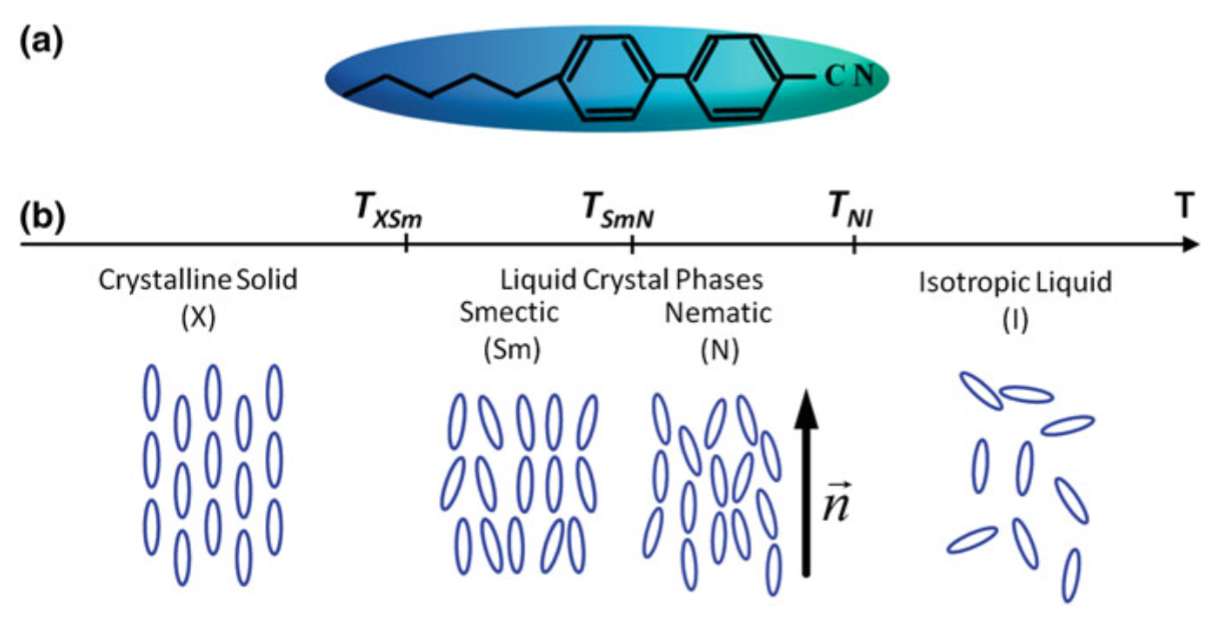
\includegraphics[width=0.5\textwidth]{thermotropic_LC.png}
\caption{\textbf{(a)} Anisotropic shape of a typical liquid crystal molecule (here Pentylcyanobiphenyl), modelled as a spheroid. \textbf{(b)} Different crystal phases and domains of existence. Vector $\vec{n}$ denotes the local director field along which the orientations of the particles are aligned in the non-isotropic phases. \textit{source:} \cite{sengupta2013topological}, Figure 2.1}
\label{thermotropic_LC}
\end{figure}

From the least ordered to the most ordered, these phases are:
\begin{description}
\item[$\bm{T > T_{NI}}$:] the isotropic phase, in which the molecules are randomly oriented and positioned;
\item[$\bm{T_{SmN} < T < T_{NI}}$:] the nematic phase, in which the molecules are randomly positioned but are on average aligned with the vector $\vec{n}$, called the director, hence displaying an orientational order;
\item[$\bm{T_{XSm} < T < T_{SmN}}$:] the smectic phase, in which the molecules are segregated into planes and conserve the orientational order of the nematic phase;
\item[$\bm{T < T_{XSm}}$:] the crystalline solid, in which the molecules are perfectly ordered, both in orientation and position.
\end{description}
To distinguish the isotropic and nematic phases, and also quantify the orientational order in the nematic phase, we need to introduce a nematic order parameter.\\

Consider a packing of identically shaped particles. For a matter of simplicity, we will assume these particles have a symmetry axis, therefore for any given particle there exists $\vec{I} \in \mathbb{S}^2$ such that the particle has cylindrical symmetry around $\vec{I}$. First of all, we introduce the orientation descriptor
\begin{equation}
\bm{\sigma}(\vec{I}) = \frac{1}{2}\left(3\vec{I}\otimes\vec{I} - \mathbbm{1}\right)
\label{orientation_descriptor}
\end{equation}
such that $\vec{I}$ is an eigenvector of $\bm{\sigma}(\vec{I})$ associated to the eigenvalue $1$ and $\bm{\sigma}(\vec{I})$ is an homothety of ratio $-1/2$ on $\text{span}(\vec{I})^{\perp}$, thus leading to $\text{tr}(\bm{\sigma}(\vec{I})) = 0$. Moreover, we can notice that, by definition, $\bm{\sigma}(\vec{I})$ is real and symmetric.\\

We then introduce the probability distribution function of orientation, $f(\vec{I})$, such that the probability of a given particle to have its axis of symmetry aligned with $\vec{I}$ is $f(\vec{I})d^2\vec{I}$. Since $f$ is a probability distribution function, it must satisfy the following condition
\begin{equation}
\int_{\mathbb{S}^2} d^2\vec{I}~ f(\vec{I}) = 1
\label{normalisation_f}
\end{equation}
We finally introduce the order parameter tensor $\bm{Q}$ given by
\begin{equation}
\bm{Q} = \int_{\mathbb{S}^2} d^2\vec{I}~ f(\vec{I}) \bm{\sigma}(\vec{I}) = <\bm{\sigma}(\vec{I})>
\label{order_parameter_tensor}
\end{equation}
which satisfies $\text{tr}(\bm{Q})=0$, since $\forall \vec{I}\in\mathbb{S}^2,~ \text{tr}(\bm{\sigma}(\vec{I})) = 0$, and is also real and symmetric.\\

By application of the spectral theorem we have that $\bm{Q}$ is diagonalisable in an orthonormal triad. We denote $S$ its greatest eigenvalue and $\vec{n}$ the associated eigenvector, and $\vec{e_1}$ and $\vec{e_2}$ two other eigenvectors of $\bm{Q}$ which form an orthonormal triad with $\vec{n}$. Since $\text{tr}(\bm{Q})=0$, there exists $B$ such that $\bm{Q}\vec{e_1}=(B-S)/2~\vec{e_1}$ and $\bm{Q}\vec{e_2}=-(B+S)/2~\vec{e_2}$. With all these objects being introduced, we can now rewrite $\bm{Q}$ as
\begin{equation}
\bm{Q} = \frac{1}{2}S\left(3\vec{n}\otimes\vec{n} - \mathbbm{1}\right) + \frac{1}{2}B\left(\vec{e_1}\otimes\vec{e_1} - \vec{e_2}\otimes\vec{e_2}\right)
\label{order_parameter_tensor_S}
\end{equation}
In the case of uniaxial nematic, \textit{i.e.} when there is a single preferred direction of orientation, we have $B=0$. \cite{sengupta2013topological} We will only consider this case from now on.\\

We can now show that $\vec{n}$ is the director, introduced in Figure \ref{thermotropic_LC}, and $S$ is the nematic order parameter we have been looking for. First of all, we have to determine the relation between $S$ and $f$. We can notice that
\begin{align*}
\bm{\sigma}(\vec{I})\vec{n} &= \frac{1}{2}\left(3\vec{I}\otimes\vec{I}-\mathbbm{1}\right)\vec{n} = \frac{1}{2}\left(3\left(\vec{I}\cdot\vec{n}\right)\vec{I} - \vec{n}\right)\\
&= \underbrace{\frac{1}{2}\left(3\left(\vec{I}\cdot\vec{n}\right)^2 - 1\right)}_{P_2(\vec{I}\cdot\vec{n})}\vec{n} + a(\vec{I}) \vec{e_1} + b(\vec{I})\vec{e_2} 
\end{align*}
where $P_2$ is the second Legendre polynomial. Therefore, with
\begin{align*}
S\vec{n} = \bm{Q}\vec{n} &= \int_{\mathbb{S}^2} d^2\vec{I}~ f(\vec{I}) \bm{\sigma}(\vec{I})\vec{n}\\
&= \int_{\mathbb{S}^2} d^2\vec{I}~ f(\vec{I}) P_2(\vec{I}\cdot\vec{n})\vec{n} + \int_{\mathbb{S}^2} d^2\vec{I}~ f(\vec{I}) a(\vec{I}) \vec{e_1} + \int_{\mathbb{S}^2} d^2\vec{I}~ f(\vec{I}) b(\vec{I}) \vec{e_2}
\end{align*}
and the fact that $\vec{n}$, $\vec{e_1}$ and $\vec{e_2}$ forms an orthonormal triad, it follows that
\begin{equation}
S = \int_{\mathbb{S}^2} d^2\vec{I}~ f(\vec{I}) P_2(\vec{I}\cdot\vec{n})
\label{S_f}
\end{equation}
We have that ${P_2}_{|[-1;1]}(x)$ is a parabola with a minimum in 0 and equal maximum in -1 and 1, therefore we can interpret $S$ in Equation \ref{S_f} as a measure of how well the particles are aligned with $\vec{n}$. We can also notice that in an isotropic phase for which $f$ is a flat probability distribution, $f(\vec{I}) = f_0 = 1/4\pi$ with Equation \ref{normalisation_f}, we have
\begin{align*}
S &= \int_{\mathbb{S}^2} d^2\vec{I}~ f_0 P_2(\vec{I}\cdot\vec{n}) = \frac{1}{4\pi} \cancelto{0}{\int_{\mathbb{S}^2} d^2\vec{I}~ P_2(\vec{I}\cdot\vec{n})}\\
&= 0
\end{align*}
thus indicating that $S=0$ for an isotropic phase. We have then finally showed that $S$ is the correct nematic order parameter associated to the director $\vec{n}$.

\subsection{Nematic order in static packings of spheroids}

We want to investigate the existence of a nematic order in static packings of spheroids. This investigation has recently been led by Nascimento \textit{et al.} \cite{nascimento2017density}, also inspired by the work of Onsager. We will here develop their calculations and perform the relevant numerical calculations.

\subsubsection{Free energy}

The first step to our journey is to calculate the free energy $F$ -- or equivalently the free energy density $\mathcal{F}=F/V$ with $V$ the volume of the system -- of the packing as a function of the probability distribution of orientation $f$, so that the minimisation of $F$ -- or $\mathcal{F}$ -- will enable us to determine $f$ and consequently the nematic order parameter $S$.\\

Consider $N$ identical spheroids in a volume V, we will denote $\rho_0=N/V$ the number density of the spheroids considered homogeneous in the whole packing and $v_0$ their volume. We consider that two spheroids $i$ and $j$ interact with the following potential
\begin{equation}
U_{ij} = \begin{cases} +\infty &\text{ if } i \text{ and } j \text{ interpenetrate,} \\ 0 & \text{ otherwise.}\end{cases}
\label{interacting_potential}
\end{equation}
modeling hard-core interactions.\\

% Therefore, within a multiplicative constant which only depends on the mass and moments of inertia of the spheroids, as well as the thermodynamic beta $\beta=1/k_BT$ and the volume $V$, the partition function $Z$ of the system can expressed in the canonical ensemble as
% \begin{equation}
% Z = \frac{1}{N!} \underbrace{\int_{\Omega^N} d^5\bm{q}_1\ldots d^5\bm{q}_N \exp\left(-\beta \sum_{i\leq i<j\leq N} U_{ij}\right)}_{G_N} \label{first_Z}
% \end{equation}
% with $d^5\bm{q}=d^2\vec{I}d^3\vec{r}$ where $\vec{r} \in \mathcal{B}$ denotes the position of the centre of a given particle and $\mathcal{B}$ the physical space accessible to the particles.\\

% Our first hypothesis will be that the $N$ integral in Equation \ref{first_Z} can be rewritten as
% \begin{align*}
% G_N = \left<\int_{\Omega} d^5\bm{q}_1 \exp\left(-\beta\sum_{i=2}^N U_{1i}\right)\right>^N
% \end{align*}
% where the average is computed relative to the probability distribution of the positions and orientations of the particles $2$ to $N$. Equivalently, we can write
% \begin{align*}
% G_N = \left(\int_{\Omega}d^5\bm{q}_1 (1 - W(\bm{q}_1))\right)^N
% \end{align*}
% where
% \begin{equation}
% W(\bm{q}_1) = \left<1 - \exp\left(-\beta\sum_{i=2}^NU_{1i}\right)\right>
% \end{equation}
% can be interpreted, given the potential $U_{ij}$ in equation \ref{interacting_potential}, as the average excluded volume, \textit{i.e.} $W(\bm{q}_1)=\frac{N}{V}v_{\text{eff}}$ where $v_{\text{eff}}$ is the average volume effectively occupied by one particle. According to the authors of \cite{nascimento2017density}, this comparison enables us to write
% \begin{equation}
% \begin{aligned}
% v_{\text{eff}} &= \lambda V_{\text{exc}}\\
% W(\bm{q}_1) &= \lambda \int_{\Omega} d^5\bm{q}_2~ \rho(\bm{q}_2) \left(1 - \exp\left(-\beta U_{12}\right)\right)
% \end{aligned}
% \end{equation}
% where $V_{\text{exc}}$ is the pair excluded excluded volume, $\lambda$ a parameter which will be considered as a constant, and $\rho(\bm{q}_2)$ the density of state of particle 2.\\

% Therefore, within an additive constant, we have
% \begin{align*}
% F &= -\frac{1}{\beta} \ln Z\\
% &= -\frac{1}{\beta} \ln\frac{1}{N!} \left(\int_{\Omega} d^5\bm{q}~ (1 - W(\bm{q}))\right)^N
% \end{align*}
% which, by assumption that $\rho(\bm{q})$ is a slowly varying function of $\bm{q}$ \cite{nascimento2017density}, leads to
% \begin{align*}
% F &= \frac{1}{\beta} \left[\int_{\Omega} d^5\bm{q}~ \rho(\bm{q})\ln\rho(\bm{q}) - \int_{\Omega} d^5\bm{q}~ \rho(\bm{q})\ln(1-W(\bm{q}))\right]\\
% &= \frac{1}{\beta}\left[\int_{\Omega} d^5\bm{q}~ \rho(\bm{q})\ln\rho(\bm{q}) - \ln\left(1 - \lambda \int_{\Omega} d^5\bm{q^{\prime}}~ \rho(\bm{q^{\prime}}) \left(1-\exp\left(-\beta U_{12}\right)\right)\right)\right]
% \end{align*}
% for which we can apply our last hypothesis
% \begin{equation}
% \rho(\bm{q}) = \rho_0 f(\vec{I})
% \label{density_function_space_orientation}
% \end{equation}
% then, by integration over the physical space, where we notice
% \begin{align*}
% V_{\text{exc}}(\vec{I}_1,\vec{I}_2) = \int_{\mathcal{B}} d^3\vec{r}_{12}~ \left(1-\exp\left(-\beta U_{12}(\vec{r}_{12},\vec{I}_1,\vec{I}_2)\right)\right)
% \end{align*}
% we finally get

Authors of \cite{nascimento2017density} showed that the free energy density of the packing has the following expression within an additive constant
\begin{equation}
\begin{aligned}
\mathcal{F} = \frac{F}{V} = - \frac{1}{\beta}\rho_0 \Bigg[- \ln\rho_0 &\underbrace{-\int_{\mathbb{S}^2} d^2\vec{I}~ f(\vec{I})\ln f(\vec{I})}_{\encircle{1}}\\
&+ \underbrace{\int_{\mathbb{S}^2} d^2\vec{I} f(\vec{I}) \ln\left(1-\lambda\rho_0\int_{\mathbb{S}^2}d^2\vec{I}^{\prime}~ f(\vec{I}^{\prime})V_{\text{exc}}(\vec{I},\vec{I}^{\prime})\right)}_{\encircle{2}}\Bigg]
\end{aligned}
\label{free_energy_1_2}
\end{equation}
where $V_{\text{exc}}(\vec{I},\vec{I^{\prime}})$ is the pair excluded excluded volume between two spheroids with symmetry axis along $\vec{I}$ and $\vec{I^{\prime}}$, and $\lambda$ is a parameter which will be considered as a constant.\\

Equation \ref{free_energy_1_2} contains all the physics of the problem. Term $\encircle{1}$ represents the orientational entropy, while term $\encircle{2}$ represents the effect of excluded volume. \cite{priestly2012introduction} At low density, the effects of excluded volume are negligible, we thus have to maximise the orientational entropy in order to minimise the free energy, hence the isotropic phase. At higher density, when particles are more closely packed, the effects of excluded volume are predominant, particles thus have to align in order to minimise the excluded volume and minimise the free energy, hence the nematic phase. A phase transition between the isotropic and nematic is then to be expected at a given density.\\

We can now get on with the minimisation of the free energy. We must first provide an expression for the excluded volume. Recent work by Piastra and Virga \cite{piastra2015explicit}, summarised in Appendix A of \cite{nascimento2017density} for spheroids, showed that for spheroids with symmetry axis aligned with $\vec{I}$ and $\vec{I^{\prime}}$ we can write
\begin{equation}
V_{\text{exc}}(\vec{I},\vec{I^{\prime}}) = C - \frac{2}{3}D\bm{\sigma}(\vec{I}):\bm{\sigma}(\vec{I^{\prime}})
\label{expression_excluded_volume}
\end{equation}
where $C$ and $D$ are constants determined by the aspect ration of the spheroids and $:$ denotes the double dot product such that
\begin{align*}
A = \sum_i \vec{a_i}\otimes\vec{b_i},~ B=\sum_j\vec{c_j}\otimes\vec{b_j} \Rightarrow A:B = B:A = \sum_i\sum_j (\vec{a_i}\cdot\vec{d_j})(\vec{b_i}\cdot\vec{c_j})
\end{align*}
For a matter of simplicity, we will denote $c=\lambda C$ and $d=\lambda D$. We can now rewrite equation \ref{free_energy_1_2} as
\begin{align*}
\mathcal{F} = \frac{1}{\beta} \rho_0 \Bigg[\ln\rho_0 &+ \int_{\mathbb{S}^2}d^2\vec{I}~ f(\vec{I})\ln f(\vec{I})\\
&- \int_{\mathbb{S}^2} d^2\vec{I}~f(\vec{I})\ln\left(1 - \rho_0\int_{\mathbb{S}^2}d^2\vec{I^{\prime}}~f(\vec{I^{\prime}})\left(c - \frac{2}{3}d\bm{\sigma}(\vec{I}):\bm{\sigma}(\vec{I^{\prime}})\right)\right)\Bigg]
\end{align*}
where
\begin{align*}
&\int_{\mathbb{S}^2}d^2\vec{I^{\prime}}~f(\vec{I^{\prime}})\left(c - \frac{2}{3}d\bm{\sigma}(\vec{I}):\bm{\sigma}(\vec{I^{\prime}})\right)\\
= &c\cancelto{1}{\int_{\mathbb{S}^2}d^2\vec{I^{\prime}}~~~ f(\vec{I^{\prime}})}~ - \frac{2}{3} d \bm{\sigma}(\vec{I}):\underbrace{\int_{\mathbb{S}^2}d^2\vec{I^{\prime}}~f(\vec{I^{\prime}})\bm{\sigma}(\vec{I^{\prime}})}_{=\bm{Q}}
\end{align*}
then, with the following dimensionless parameter
\begin{equation}
\phi = \frac{\rho_0 c - 1}{\rho_0 d}
\end{equation}
introduced in \cite{nascimento2017density}, we finally get
\begin{equation}
\begin{aligned}
\mathcal{F} = \frac{1}{\beta}\rho_0 \Bigg[\ln\rho_0 &+ \int_{\mathbb{S}^2}d^2\vec{I}~ f(\vec{I})\ln f(\vec{I}) \\
&- \int_{\mathbb{S}^2}d^2\vec{I}~f(\vec{I})\ln\left(\frac{2}{3}\bm{\sigma}(\vec{I}):\int_{\mathbb{S}^2}d^2\vec{I^{\prime}}~f(\vec{I^{\prime}})\bm{\sigma}(\vec{I^{\prime}}) - \phi\right)\Bigg]
\end{aligned}
\label{free_energy_to_minimise}
\end{equation}
which has to be minimised with respect to $f(\vec{I})$ with the constraint of Equation \ref{normalisation_f} written as
\begin{equation}
\mathcal{G} = \int_{\mathbb{S}^2}d^2\vec{I}~f(\vec{I}) - 1 = 0
\end{equation}
Therefore, if $f(\vec{I})$ minimises $\mathcal{F}$, we have for any infinitely small $\delta f(\vec{I})$
\begin{equation}
\mathcal{F}\left(f(\vec{I})+\delta f(\vec{I})\right) - \mathcal{F}\left(f(\vec{I})\right) + \mu\left(\mathcal{G}\left(f(\vec{I})+\delta f(\vec{I})\right) - \mathcal{G}\left(f(\vec{I})\right)\right) = 0
\label{minimisation_F_G}
\end{equation}
where $\mu$ is a Lagrange multiplier.\\

We have
\begin{align*}
&\int_{\mathbb{S}^2}d^2\vec{I}~(f(\vec{I})+\delta f(\vec{I}))\ln(f(\vec{I})+\delta f(\vec{I})) - \int_{\mathbb{S}^2}d^2\vec{I}~f(\vec{I})\ln f(\vec{I})\\
= &\int_{\mathbb{S}^2} d^2\vec{I}~\delta f(\vec{I})(\ln f(\vec{I}) + 1)
\end{align*}
and within an additional term of order $\mathcal{O}(\delta f^2)$
\begin{align*}
&\int_{\mathbb{S}^2}d^2\vec{I}~(f(\vec{I})+\delta f(\vec{I}))\ln\left(\frac{2}{3}\bm{\sigma}(\vec{I}):\int_{\mathbb{S}^2}d^2\vec{I^{\prime}}~(f(\vec{I^{\prime}})+\delta f(\vec{I^{\prime}}))\bm{\sigma}(\vec{I^{\prime}}) - \phi\right)\\
&- \int_{\mathbb{S}^2}d^2\vec{I}~f(\vec{I})\ln\left(\frac{2}{3}\bm{\sigma}(\vec{I}):\int_{\mathbb{S}^2}d^2\vec{I^{\prime}}~f(\vec{I^{\prime}})\bm{\sigma}(\vec{I^{\prime}}) - \phi\right)\\
= &\int_{\mathbb{S}^2}d^2\vec{I}~\delta f(\vec{I}) \ln\Bigg(\frac{2}{3}\bm{\sigma}(\vec{I}):\underbrace{\int_{\mathbb{S}^2}d^2\vec{I^{\prime}}~f(\vec{I^{\prime}})\bm{\sigma}(\vec{I^{\prime}})}_{\bm{Q}}-\phi\Bigg)\\
&+ \int_{\mathbb{S}^2} d^2\vec{I}~\delta f(\vec{I}) \bm{\sigma}(\vec{I}):\Bigg(\int_{\mathbb{S}^2}d^2\vec{I^{\prime}}~f(\vec{I^{\prime}})\frac{\frac{2}{3}\bm{\sigma}(\vec{I^{\prime}})}{\frac{2}{3}\bm{\sigma}(\vec{I^{\prime}}):\underbrace{\int_{\mathbb{S}^2}d^2\vec{I^{\prime\prime}}~f(\vec{I^{\prime\prime}})\bm{\sigma}(\vec{I^{\prime\prime}})}_{\bm{Q}}-\phi}\Bigg)
\end{align*}
and finally
\begin{align*}
\mathcal{G}\left(f(\vec{I})+\delta f(\vec{I})\right) - \mathcal{G}\left(f(\vec{I})\right) = \int_{\mathbb{S}^2} d^2\vec{I}~\delta f(\vec{I})
\end{align*}
thus, with
\begin{equation}
\frac{2}{3}\bm{\sigma}(\vec{I}):\bm{Q} = SP_2(\vec{I}\cdot\vec{n})
\label{sigmaQ}
\end{equation}
Equation \ref{minimisation_F_G} becomes
\begin{equation}
\begin{aligned}
\int_{\mathbb{S}^2}d^2\vec{I}~\delta f(\vec{I}) \Bigg(&\ln f(\vec{I}) + 1 - \ln\left(SP_2(\vec{I}\cdot\vec{n})-\phi\right)\\
&- \bm{\sigma}(\vec{I}):\left(\int_{\mathbb{S}^2}d^2\vec{I^{\prime}}~f(\vec{I^{\prime}})\frac{\frac{2}{3}\bm{\sigma}(\vec{I^{\prime}})}{SP_2(\vec{I}\cdot\vec{n})-\phi}\right)+\mu \Bigg) = 0
\end{aligned}
\label{minimisation_F}
\end{equation}
which has to be verified for any choice of $\delta f(\vec{I})$, implying that the part between parenthesis in the integrand must be equal to 0.\\

We introduce
\begin{equation}
\bm{\psi} = \int_{\mathbb{S}^2}d^2\vec{I}~ f(\vec{I})\frac{\frac{2}{3}\bm{\sigma}(\vec{I})}{SP_2(\vec{I}\cdot\vec{n})-\phi} = \psi(\vec{n}\otimes\vec{n}-\frac{1}{3}\mathbbm{1})
\label{psi_def}
\end{equation}
such that
\begin{align*}
\bm{\sigma}(\vec{I}):\bm{\psi} = \psi P_2(\vec{I}\cdot\vec{n})
\end{align*}
and that the function $f(\vec{I})$ which satisfies Equation \ref{minimisation_F} is
\begin{equation}
\begin{aligned}
f(\vec{I}) = \begin{cases} \frac{(SP_2(\vec{I}\cdot\vec{n})-\phi)e^{\psi P_2(\vec{I}\cdot\vec{n})}}{\int_{\mathbb{S}^2_+}d^2\vec{I^{\prime}}~(SP_2(\vec{I^{\prime}}\cdot\vec{n})-\phi)e^{\psi P_2(\vec{I^{\prime}}\cdot\vec{n})}} &\text{ if } SP_2(\vec{I}\cdot\vec{n})-\phi > 0,\\ 0 & \text{ otherwise.} \end{cases}
\end{aligned}
\label{f_I_equilibrium}
\end{equation}
where $\mathbb{S}^2_+ = \{\vec{I}\in\mathbb{S}^2,~SP_2(\vec{I}\cdot\vec{n}) - \phi >0\}$. We have that the only relevant variable is $x\equiv\vec{I}\cdot\vec{n}$, therefore by integration over the other components of $\vec{I}$ and by noticing that the integrand in the denominator is an even function of $x$, we get
\begin{equation}
\begin{aligned}
f(x) = \frac{1}{4\pi}\begin{cases} \frac{(SP_2(x)-\phi)e^{\psi P_2(x)}}{\int_{S_+}dx^{\prime}~(SP_2(x^{\prime})-\phi)e^{\psi P_2(x^{\prime})}} &\text{ if } SP_2(x)-\phi > 0,\\ 0 & \text{ otherwise.} \end{cases}
\end{aligned}
\label{self_consistent_f}
\end{equation}
where $S_+ =\{x\in[0;1], SP_2(x)-\phi>0\}$. Rather than solving this self-consistent equation for $f(x)$, we use Equations \ref{S_f} and \ref{psi_def} in Equation \ref{self_consistent_f}, and with $x_0$ the positive root of
\begin{equation}
SP_2(x_0) - \phi = 0
\label{x0_root}
\end{equation}
we write
\begin{equation}
S = \frac{\int_{S_+}dx~P_2(x)(P_2(x)-P_2(x_0))e^{\psi P_2(x)}}{\int_{S_+}dx~(P_2(x)-P_2(x_0))e^{\psi P_2(x)}}
\label{S_eq}
\end{equation}
\begin{equation}
\frac{1}{\psi} = \frac{\int_{S_+}dx~P_2^2(x)e^{\psi P_2(x)}}{\int_{S_+}dx~P_2(x)e^{\psi P_2(x)}} - P_2(x_0)
\label{psi_eq}
\end{equation}
for which $S_+$ is then given by
\begin{align*}
S_+ = \begin{cases} [x_0;1] &\text{ if } S>0,\\ [0;x_0] &\text{ if } S<0.\end{cases}
\end{align*}

\subsubsection{Equilibrium nematic order parameter}

To get the equilibrium nematic order parameter $S$ as a function of the order parameter $\phi(\rho_0)$, we take a $\psi\in]-\infty;+\infty[$ and solve Equation \ref{psi_eq} for $x_0$, then find the corresponding $S>0$ and $S<0$ with Equation \ref{S_eq} and finally the corresponding $\phi$ with Equation \ref{x0_root}.\\

To determine the stability of the equilibrium solutions, we need to know for each $\phi$ the local convexity of the free energy in the vicinity of the corresponding equilibrium nematic order parameters $S^*(\phi)$. Let us first notice with Equation \ref{f_I_equilibrium} that
\begin{align*}
\int_{\mathbb{S}^2}d^2\vec{I}~&f(\vec{I})\ln f(\vec{I}) = \underbrace{\int_{\mathbb{S}^2_+} d^2\vec{I}~ f(\vec{I})\psi P_2(\vec{I}\cdot\vec{n})}_{\psi S} + \int_{\mathbb{S}^2_+} d^2\vec{I}~ f(\vec{I})\ln(SP_2(\vec{I}\cdot\vec{n})-\phi)\\
&- \underbrace{\int_{\mathbb{S}^2}d^2\vec{I}~ f(\vec{I}) \ln\int_{\mathbb{S}^2_+}d^2\vec{I^{\prime}}~(SP_2(\vec{I^{\prime}}\cdot\vec{n})-\phi)e^{\psi P_2(\vec{I^{\prime}}\cdot\vec{n})}}_{\ln\int_{\mathbb{S}^2_+}d^2\vec{I^{\prime}}~(SP_2(\vec{I^{\prime}}\cdot\vec{n})-\phi)e^{\psi P_2(\vec{I^{\prime}}\cdot\vec{n})}}
\end{align*}
Therefore, with Equations \ref{free_energy_to_minimise} and \ref{sigmaQ}, we have the following expression within an additive constant for the free energy density
\begin{equation}
\begin{aligned}
\mathcal{F} = \frac{1}{\beta}\rho_0\left(\psi S - \ln\int_{\mathbb{S}^2_+}d^2\vec{I}~(SP_2(\vec{I}\cdot\vec{n})-\phi)e^{\psi P_2(\vec{I}\cdot\vec{n})}\right)
\end{aligned}
\label{free_energy_for_curvature}
\end{equation}
We can then compute the first and second partial derivatives of $\mathcal{F}$ with respect to $S$ to determine the stability of the solutions.\\

% We will classify them as:
% \begin{description}
% \item[\textbf{unstable}:] $\left.\frac{\partial}{\partial S}\mathcal{F}\right|_{S^*(\phi)} \neq 0$ or $\left.\frac{\partial^2}{\partial S^2}\mathcal{F}\right|_{S^*(\phi)} < 0$,
% \item[\textbf{metastable}:] $\left.\frac{\partial}{\partial S}\mathcal{F}\right|_{S^*(\phi)} = 0$, $\left.\frac{\partial^2}{\partial S^2}\mathcal{F}\right|_{S^*(\phi)} > 0$ and there exists an other equilibrium nematic order parameter for which the free energy is lower,
% \item[\textbf{stable}:] $\left.\frac{\partial}{\partial S}\mathcal{F}\right|_{S^*(\phi)} = 0$, $\left.\frac{\partial^2}{\partial S^2}\mathcal{F}\right|_{S^*(\phi)} > 0$ and there does not exist an other equilibrium nematic order parameter for which the free energy is lower.\\
% \end{description}

We solved the minimisation equation for $\mathcal{F}$, determined the couples $(\phi,S)$ of equilibrium solutions and computed the local convexity of $\mathcal{F}$ with Wolfram \textsc{MATHEMATICA}. All the code which has been developed for this task is available on the GitHub repository \href{https://github.com/yketa/M2_PT_project}{yketa/M2\_PT\_project}. We are mainly interested in stable solutions with $S > 0$, therefore we only show here the results for the conditions $S > 0$ and $\psi \in ]0;+\infty[$, and $S = 0$ and $\psi = 0$ which is also an equilibrium solution $\forall\phi < 0$ according to equations \ref{S_eq} and \ref{psi_eq}. Results are presented in Figure \ref{Sphi}.

\begin{figure}[h!]
\centering
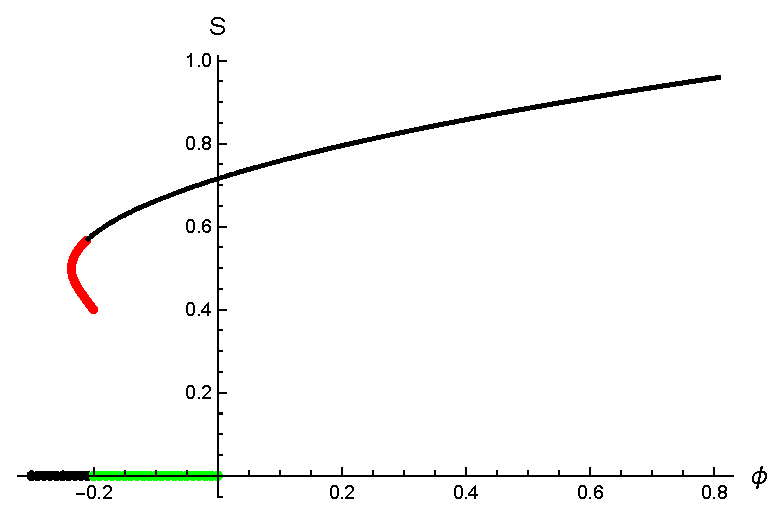
\includegraphics[width=0.5\textwidth]{figures/figs/FinalPlot.eps}
\caption{Nematic order parameter $S$ as a function of $\phi$. Black curves represent stable states, red curve represents metastable states and green curve represents unstable states.}
\label{Sphi}
\end{figure}

From our data, we get that the stable solution for $\phi < \phi_{NI} \sim -0.211$ is $S=0$ while the stable solution for $\phi > \phi_{NI}$ is $S > S_{NI} \sim 0.567$. Therefore, there is a phase transition at $\phi=\phi_{NI}$ between an isotropic and a nematic phase. There is a discontinuity in the order parameter $S$ at this transition, which is then a first-order phase transition.\\

Our results are a bit different from the paper, where the authors got $\phi_{NI,\text{th.}} = -0.224$ and $S_{NI,\text{th.}} = 0.545$. Moreover, we do not observe a metastable part in the $S>0$ curve. We believe these differences are due to numerical errors in the successive operations we have performed.

% \addcontentsline{toc}{section}{References}
\bibliographystyle{unsrtnat}
\bibliography{references/biblio}
{\renewcommand{\bibname}{References}\bibliography{references/biblio}}

\end{document}

% \end{cbunit}